\chap{Un robot de compagnie}\label{ch.pet}

Un \emph{robot autonome} adopte un comportement spécifique en fonction de la situation dans laquelle il se trouve.
Il réussi à réagir grâce au \textit{feedback}, littéralement de l'information en retour.
Il faut donc que le robot puisse «\,voir\,» le monde qui l'entoure pour pouvoir y réagir.

\sect{Thymio vous obéit}

Pour commencer, nous allons programmer Thymio pour qu'il vous obéisse.
Normalement, le robot restera sur place sans bouger ; quand il détectera votre main devant lui, il bougera en sa direction.

Thymio a cinq capteurs de distance horizontaux à l'avant et deux à l'arrière.
Ils sont similaires à ceux qui se trouve sous Thymio et que nous avons utilisé au \cref{c.moving}.
Avancez votre main en direction des capteurs à l'avant de Thymio, vous verrez une lumière rouge apparaître à côté du capteur qui vous aura détecté, comme sur la \cref{fig.detect}.

\begin{figure}
\begin{center}
\gr{detect}{.6}
\caption{L'avant de Thymio. Deux doigts sont détectés par les capteurs. avant.}\label{fig.detect}
\end{center}
\end{figure}

Le bloc \blksm{event-prox} sert à utiliser les capteurs horizontaux avants et arrières de Thymio.
Les petits carrés gris (cinq sur l'avant et deux sur l'arrière) sont utilisées comme pour les détecteurs situés sous Thymio.
En cliquant dessus, ils passent de gris à blanc, à rouge et à nouveau à gris.
Pour ce bloc, les significations des couleurs sont :

\begin{itemize}
\item \textbf{Gris} : Le détecteur n'est pas utilisé.
\item \textbf{Rouge} : L'événement associé est déclenché si un objet se trouve proche.
\item \textbf{Blanc} : L'événement associé est déclenché si aucun objet ne se trouve proche.
\end{itemize}

\importantbox[Détecteurs de sols et capteurs de distance horizontaux]{
Attention à ne pas confondre le comportement des capteurs de distance horizontaux avec celui des détecteurs de sols.
\begin{itemize}[noitemsep,nosep,leftmargin=*]
\item Pour les capteurs horizontaux, le carré blanc spécifie qu'un événement se produire s'il n'y a \emph{rien à proximité}, alors qu'un carré rouge spécifie qu'un événement se produira s'il y a \emph{quelque chose à proximité}.
\item Pour les détecteurs de sols, le carré blanc spécifie qu'un événement se produira s'il y a \emph{peu de lumière réfléchie par la surface} alors qu'un carré rouge spécifie qu'un événement se produira \emph{s'il y a beaucoup de lumière réfléchie par la surface}.
\end{itemize}
Le principe physique de ces deux types de capteurs est similaire, mais parce qu'ils sont placés différemment, leur comportement est différent.
}

Pour construire le comportement, il nous faut deux paires événement-action, comme sur la \cref{fig.follow-hand}.
Dans ce programme, vous voyez que dans la première paire, le carré central est blanc et l'action associée est que les moteurs sont arrêtés.
Ainsi, lorsque le robot ne voit rien, il ne bougera pas ; et s'il bougeait, il s'arrêtera.
Dans la deuxième paire, le carré central est rouge et les sliders du bloc action moteur sont glissés vers le haut.
Ainsi, lorsque vous amenez votre main près de l'avant du robot, un événement se produit qui fait tourner les deux moteurs assez vite et fait avancer le robot en avant.


\begin{figure}
\begin{floatrow}
	\ffigbox
	{\caption{Thymio avance vers votre main}\label{fig.follow-hand}}
	{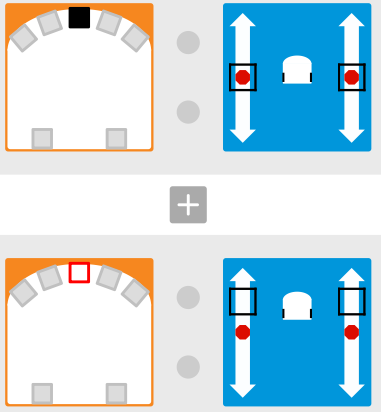
\includegraphics[width=.4\textwidth]{likes-forward}}
	\ffigbox
	{\caption{Un bulldozer à chenilles}\label{fig.bull}}
	{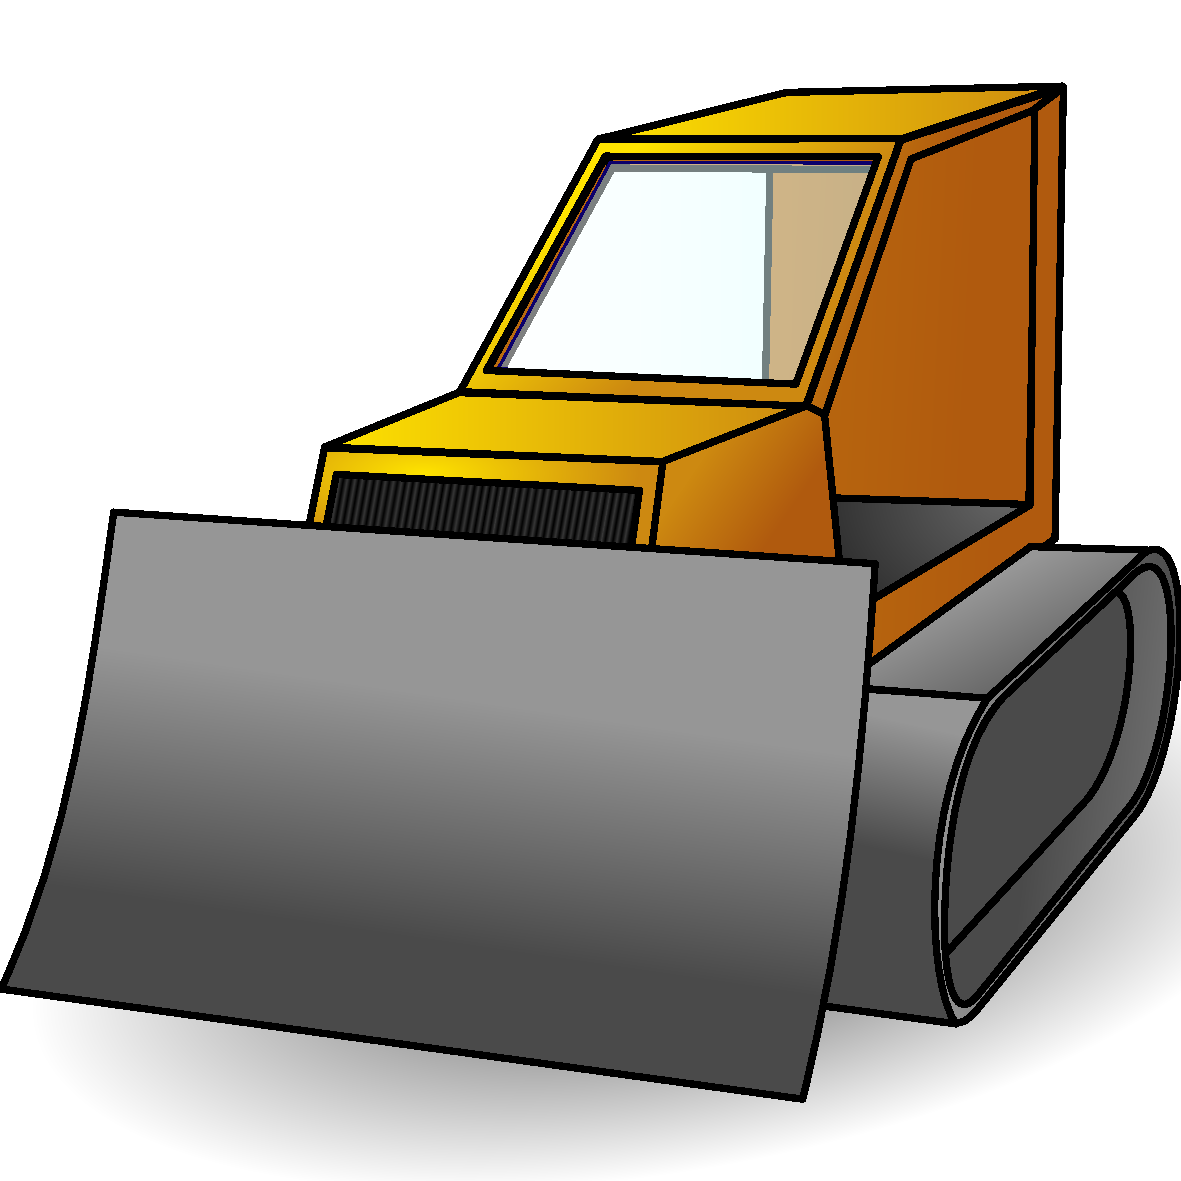
\includegraphics[width=.35\textwidth]{bulldozer}}
\end{floatrow}
\end{figure}

\sect{Faire tourner Thymio}

Thymio n'a pas un volant comme une voiture ou un guidon comme un vélo.
Comment tourne-t-il donc ? 
Pour tourner, le robot utilise une \emph{direction différentielle}, ou \emph{differential drive}, qui est  utilisée par de nombreux véhicules à chenilles comme le bulldozer sur la \cref{fig.bull}.
À la place de tourner un guidon dans la direction désirée, les chenilles ou roues gauches et droites sont commandées par des moteurs individuels à des vitesses \emph{différentes}.
Si la roue droite tourne plus vite que la roue gauche, alors le véhicule tournera à gauche, tandis que si sa roue gauche tourne plus vite que sa roue droite, il tournera à droite.

Dans VPL, en réglant le bloc action moteur avec les \textit{sliders} à des endroits différents, les roues de Thymio ne tourneront pas à la même vitesse, ce qui fera tourner le robot.
Plus la différence de vitesse est élevée, plus le virage sera serré.
Pour arriver à une grande différence de vitesses, vous pouvez faire tourner une roue en avant et l'autre en arrière.
En fait, pour tourner sur lui-même, il suffit à Thymio de faire tourner ses deux roues à la même vitesse mais dans des sens opposés !
Par exemple, dans ce bloc action moteur \blksm{differential}, le \textit{slider} gauche indique une grande vitesse en arrière, alors que le \textit{slider} droite indique une grande vitesse en avant.
Le résultat est que le robot tournera sur lui-même en direction de la gauche, comme indiqué par l'image du robot.

Expérimentez avec une paire événement-action telle que celle ci : \blkc{turning}

Si vous chargez ensuite ce programme et appuyez sur le bouton central, Thymio devrait tourner sur lui-même. Vous pouvez toujours l'arrêter en appuyant sur \blksm{stop}.

\trickbox{L'icône du Thymio au centre du bloc action moteur s'anime dès que vous réglez les \textit{sliders} pour vous donner une idée du mouvement de Thymio!}


\sect{Thymio vous aime}

Un vrai animal de compagnie ne se contente pas de s'approcher ou de s'éloigner de vous, il vous suit un peu partout! 
Pour que Thymio puisse vous suivre le plus fidèlement possible, il faudra ajouter deux paires événement-action au programme précédant.
Si Thymio vous détecte avec son capteur avant-droit, il doit tourner à droite et s'il vous détecte avec son capteur avant-gauche, il doit tourner à gauche.

{\raggedleft \hfill Programme \bu{likes.aesl}}

Une façon de faire est illustrée sur la \cref{fig.likes}.
Vous pouvez essayer différentes vitesses, le faire tourner sur lui-même ou non, afin de trouver le meilleur comportement !

\begin{figure}
	\subfigure[Thymio s'oriente face à vous]{
		\label{fig.likes}
		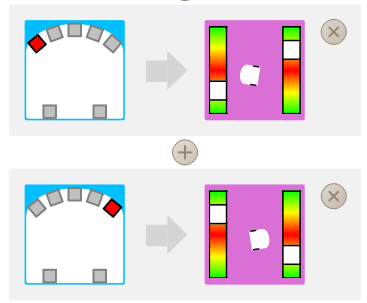
\includegraphics[width=.4\textwidth]{likes-turns}
	}
	\hfill
	\subfigure[Thymio vous évite]{
		\label{fig.hates}
		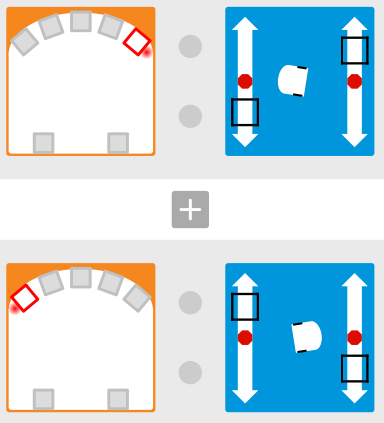
\includegraphics[width=.4\textwidth]{hates}
	}
	\caption{Programmes pour robot de compagnie}
\end{figure}

\exercisebox{\thechapter.1}{
Modifiez le comportement du robot de compagnie pour qu'il bouge en avant quand le programme est exécuté et qu'il s'arrête lorsqu'il détecte le bord de la table (ou une bande de ruban adhésif noir). \\
{\small Comme vu dans le \cref{c.moving}, beaucoup de lumière sera réfléchie par une surface blanche, et peu par une surface noire.
Vous aller devoir expérimenter avec le bloc capteurs horizontaux pour déterminer quand choisir un carré blanc et quand choisir un carré noir, en fonction du sol ou de la table sur lequel vous placez le robot.}
}

\exercisebox{\thechapter.2}{
Qu'arrive-t-il si vous changez l'ordre des paires d'événement-action utilisées à l'exercice précédent ?
}


\sect{Thymio ne vous aime pas}

Parfois, même le plus fidèle animal de compagnie n'a pas envie de vous suivre. 
Écrivez un programme qui génère ce comportement.

{\raggedleft \hfill Programme \bu{does-not-like.aesl}}

Ouvrez le programme du Thymio qui vous aime et inversez l'association des événements avec les actions, comme montré sur la \cref{fig.hates}.
Détecter un obstacle avec le capteur gauche fait tourner le robot à droite, et détecter un obstacle avec le capteur droite fait tourner le robot à gauche.

% \begin{figure}[h]
%     \centering
%     \subfigure[S'il vous détecte devant lui, il recule]{ \label{fig.recule} 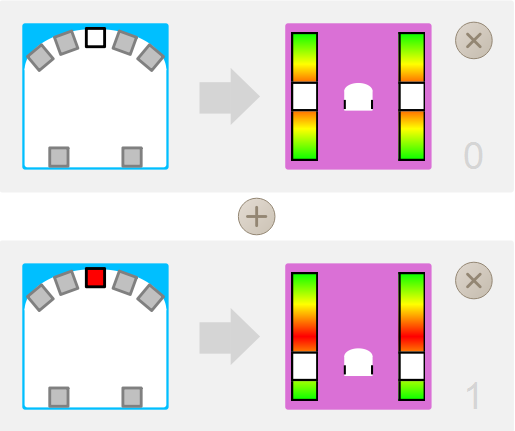
\includegraphics[width = 0.35\textwidth]{hates2}}
%     \hspace{1cm}
%     \subfigure[S'il vous détecte sur les côtés, il vous évite]{ \label{fig.evite} 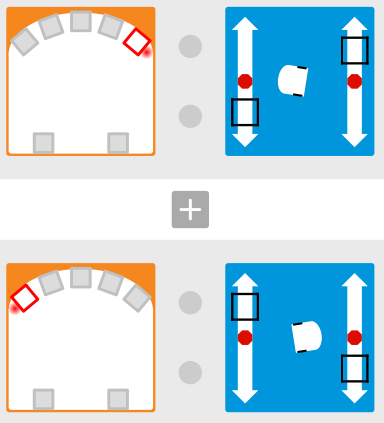
\includegraphics[width = 0.35\textwidth]{hates}}
%     \caption{Thymio vous évite et vous fuit}
%     \label{fig.recule-evite}
% \end{figure}

\exercisebox{\thechapter.3}
{
Jouez avec les différents capteurs avant de Thymio.
Les capteurs horizontaux avant sont numérotés 0, 1, 2, 3, 4 de gauche à droite.
Les capteurs arrière sont numérotés 5 pour le gauche et 6 pour le droite.
À la place d'utiliser les capteurs 0 et 4 comme jusqu'à maintenant:
\begin{itemize}[noitemsep,nosep,leftmargin=*]
\item Utilisez les capteur 1 pour tourner le robot à gauche et le 3 pour à droite.
\item Utilisez à la fois les capteurs 0 et 1 pour tourner le robot à gauche et à la fois les capteurs 3 et 4 pour tourner le robot à droite.
\item Ajouter une paire événement-action pour les capteurs arrières 5 et 6.
\end{itemize}
}

\sect{Régler les \textit{sliders} plus précisément (avancé)}

Ce n'est pas très facile de régler les \textit{sliders} précisément pour, par exemple, faire avancer Thymio tout droit.
En regardant la traduction textuelle des paires événement-action, il est possible d'ajuster plus précisément les vitesses des roues.
Le \cref{fig.textcode} montre le programme du Thymio qui vous suit, avec la traduction texte à droite.
Ce texte est écrit automatiquement quand vous éditez les paires événement-action.

\begin{figure}
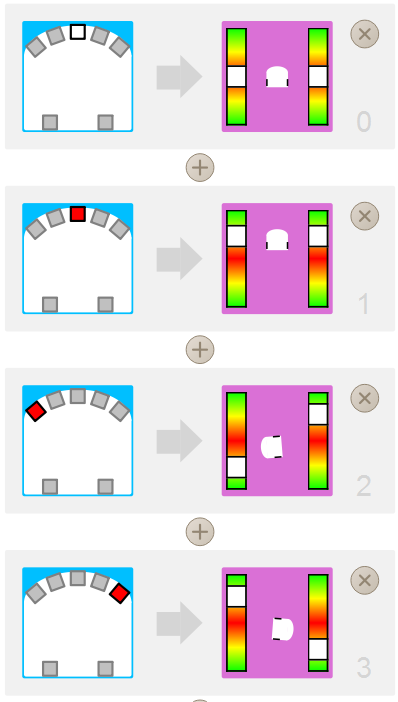
\includegraphics[width=0.3\textwidth]{follow4}
\hfill
\begin{minipage}[b]{0.6\textwidth}
\footnotesize
\begin{lstlisting}
onevent prox
	if prox.horizontal[2] < 400 then
		motor.left.target = 0
		motor.right.target = 0
	end
	if prox.horizontal[2] > 500 then
		motor.left.target = 300
		motor.right.target = 300
	end
	if prox.horizontal[0] > 500 then
		motor.left.target = -300
		motor.right.target = 300
	end
	if prox.horizontal[4] > 500 then
		motor.left.target = 300
		motor.right.target = -300
	end
\end{lstlisting}
\end{minipage}
\caption{Un programme VPL et le programme texte correspondant.}
\label{fig.textcode}
\end{figure}

La ligne \p{onevent prox} signifie que les lignes qui suivent seront exécutées lorsque la lecture des capteurs de distance (appelés \textit{proximity} et abrégés \textit{prox}) se produit (elle se produit 10 fois par seconde).

Lorsque l'événement se produit, Thymio teste la valeur des capteurs en utilisant une condition de type \p{if} \ldots \ \p{then} \ldots \ \p{end}, c'est à dire \p{si} \ldots \ \p{alors} \ldots \ \p{fin}.
Il commence par tester le capteur numéro 2 (avant centre) comme nous le voyons avec \p{prox.horizontal[2]}.
Si cette valeur est inférieure à 400, alors Thymio règle la vitesse des moteurs gauche et droite à 0 avec les instructions \p{motor.left.target = 0} et \p{motor.right.target = 0}.
Chaque bloc \p{if} \ldots \ \p{then} \ldots \ \p{end} teste un capteur spécifique et effectue ou non l'action associée, en fonction du résultat du test.
Il correspond donc à une paire événement-action:
\begin{enumerate}[start=0]
	\item teste si rien ne se trouve devant ; si c'est le cas, Thymio s'arrête.
	\item teste s'il y a quelque chose devant ; si c'est le cas, Thymio avance.
	\item teste s'il y a quelque chose à gauche ; si c'est le cas, Thymio tourne à gauche.
	\item teste s'il y a quelque chose à droite ; si c'est le cas, Thymio tourne à droite.
\end{enumerate}
Finalement, une fois que Thymio a testé tous ces capteurs, il attend le prochain événement \p{prox} et recommence ces tests, indéfiniment.
Pour apprendre comment éditer le mode texte, voir le \cref{c.next}.

\trickbox{En bougeant les \textit{sliders} des blocs d'action moteur, vous verrez les vitesses visées pour les moteurs (\p{moter.X.target}) changer par pas de 50 dans l'intervalle $-$500 à 500.
En bougeant les \textit{sliders} avec soin, vous pouvez choisir n'importe laquelle de ces valeurs.
}